\documentclass{article}

\usepackage[left=1in, right=1in, top=0.5in]{geometry}

\usepackage{graphicx}

\begin{document}

\title{Microtonal Synthesizer using custom MIDI controller and Google NSynth for timbral control}
\author{John Tronolone\and Alex Hu}
\date{}

\maketitle

\begin{abstract}
A MIDI controller that uses a grid of programmable buttons enables almost unlimited potential for exploring music in non-western tunings in a simple and visually straightforward manner. By integrating a google nsynth in this MIDI controller, a relatively unknown domain of tone and timbre may easily be explored.

The end goal would be to have a completely programmable grid of buttons with 6 rows and 31 columns, with each row having an adjustable offset in frequency like present between the strings of a guitar. This would mean that using the same hand shapes in different positions would result in the same type of chord. There will be two buttons for cycling between the tuning systems, two buttons for each row for adjusting the frequency offset. There will be red-green-blue LEDs for indicating the value of the notes, with a spectrum from red to blue indicating one full octave. As a prototype, we want to be able to support the standard 12-note octave of typical western music, 17edo (equal divisions of the octave), 24edo (esentially 12-ET with quartertones within each half step), and 31edo. A suitable microprocessor/programming solution will act as the MIDI controller, accepting inputs from the button grid and making the appropriate translations for sending microtones over MIDI for output to the nsynth. The google nsynth will accept MIDI input from the software controller, where knobs will be used to adjust the amount of each instrument present, and  other knobs will handle the remainder of synthesizer functions such as volume, attack, sustain, etc. We will forgo the touchscreen for design simplicity since it does not add much value to process of exploring the sound, knobs will be used instead. The most pressing task is to research a microprocessor solution to take input from a button matrix and match the microtone using a frequency shift on the midi note. Possible solutions include raspberry pi, arduino, teensy. Teensy has out-of-the-box MIDI support, while the arduino has more support.

\end{abstract}


\section*{Existing Solutions}

\subsection*{Custom Fret Guitars}

\begin{itemize}
	\item Some people have done custom tuning/fretting of guitars to hit certain harmonics
	\item Concept of acoustic tuning, how it “sounds.”
	\item By tuning the guitar and labeling frets in certain ways, specific notes can be achieved. This is of course very limited.
\end{itemize}

\begin{center}
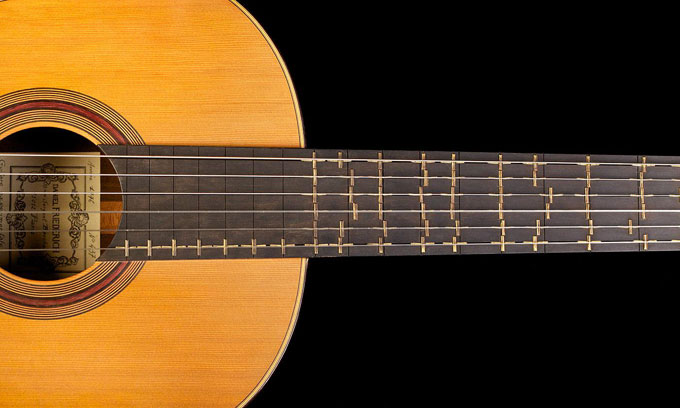
\includegraphics[width=0.5\textwidth]{mt1.jpg}
\end{center}

\subsection*{Plastic Pitch Plus Microtonal MIDI Machine}

\begin{itemize}
	\item Uses MIDI pitch bend (compatible with all MIDI synthesizers) and MIDI Tuning Standard (only works with newer 	\item hardware synthesizers).
	\item Takes input from MIDI and can output it through a connector or a computer
	\item Some issues with non-multitimbral synthesizers
	\item Controls using knobs (as shown above)
\end{itemize}

\begin{center}
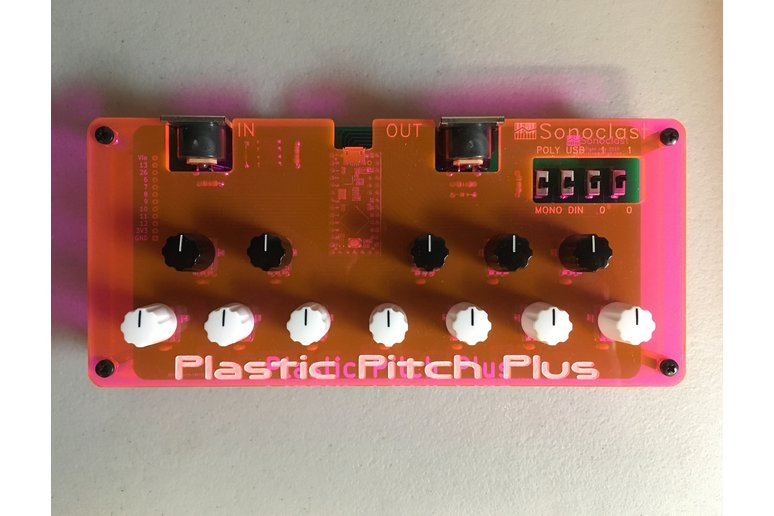
\includegraphics[width=0.5\textwidth]{mt2.jpg}
\end{center}

\subsection*{Tonal Plexus TPX 6}

\begin{itemize}
	\item Could be considered polychromatic – the pitch can be varied in both the horizontal and vertical directions.
	\item Based on how harmonics work trying to increment the frequency will eventually lead to the “same” notes, which are represented by the blue buttons on the board.
	\item No longer in production, at least as of 2016 when his post was made on the page.
	\item Capable of playing up to 200 notes with the use of buttons
	\item Creator says it represents a theory of music called the H-System
	\item Capable of programming of buttons using a control board – save the sound after tuning it
\end{itemize}

\begin{center}
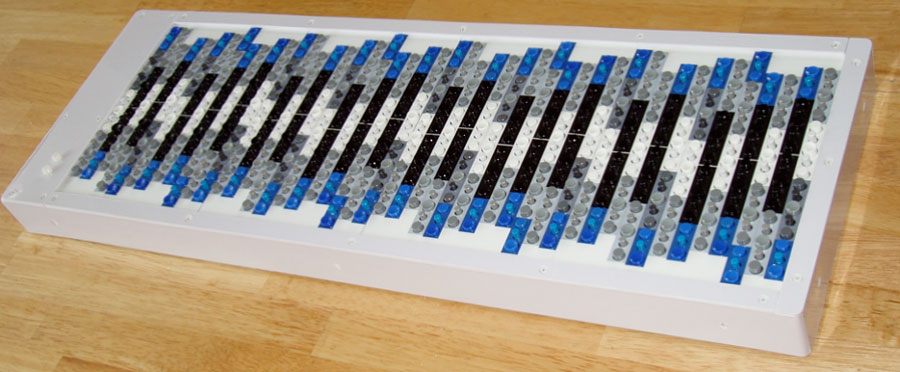
\includegraphics[width=0.5\textwidth]{mt3.jpg}
\end{center}

\subsection*{MicroZone U648}

\begin{itemize}
	\item Could be considered polychromatic
	\item Completely MIDI compatible
	\item Tuning systems and fingering could be created on keyboard with use of “Keymaps”
	\item Allows for custom ordering of keys beyond horizontal/vertical configurations
\end{itemize}

\begin{center}
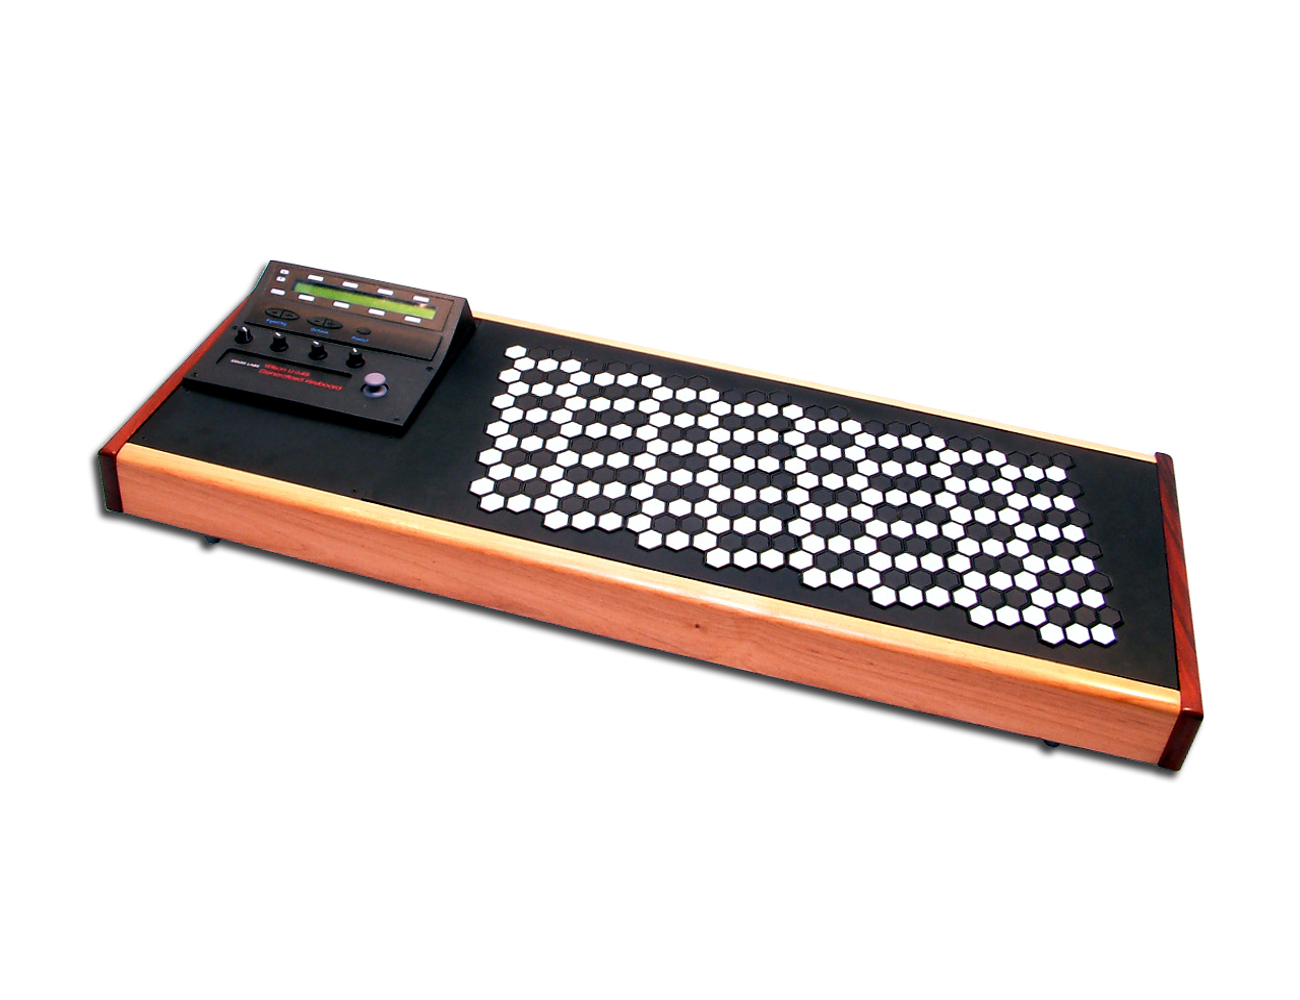
\includegraphics[width=0.5\textwidth]{mt4.jpg}
\end{center}

\subsection*{Continuum Fingerboard}

\begin{itemize}
	\item Touch sensitive horizontal pitch sweeping – can play standard 12 notes as well as notes in between by incremental adjustments of where the fingers press.
	\item Can only vary sound along the horizontal axis – it’s similar to a multi-keyed piano
	\item No tactile sense, could be difficult to play.
\end{itemize}

\begin{center}
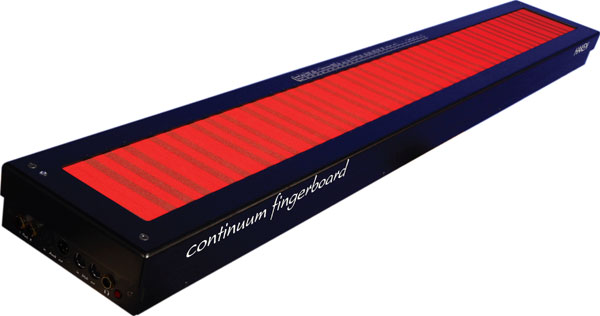
\includegraphics[width=0.5\textwidth]{mt5.jpg}
\end{center}

\subsection*{Seaboard GRAND Stage}

\begin{itemize}
	\item Similar to continuum fingerboard, arranged like piano keyboard.
	\item Could be considered easier to play with actual depth
	\item Suffers same issue with only horizontal axis control, a keyboard that can “access” notes in between.
	\item Comes equipped with many high quality synthesizer programs, which probably contributes to its high cost.
\end{itemize}

\begin{center}
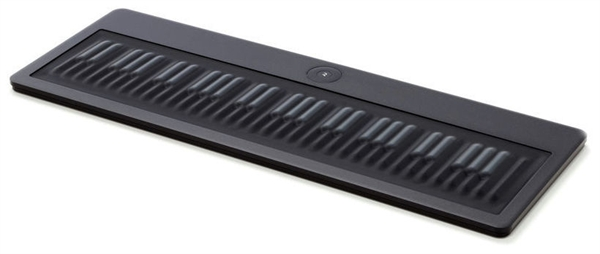
\includegraphics[width=0.5\textwidth]{mt6.jpeg}
\end{center}

\subsection*{NSynth Super}

\begin{itemize}
	\item Uses Google’s NSynth algorithm to take elements out of instruments to make new sounds
	\item Controls the instrument type as well as the type of notes coming out with the use of the 4 large knobs and the 6 small ones.
	\item Can control the “weight” of each instrument using the touch screen.
	\item Can be played via any MIDI source
\end{itemize}

\begin{center}
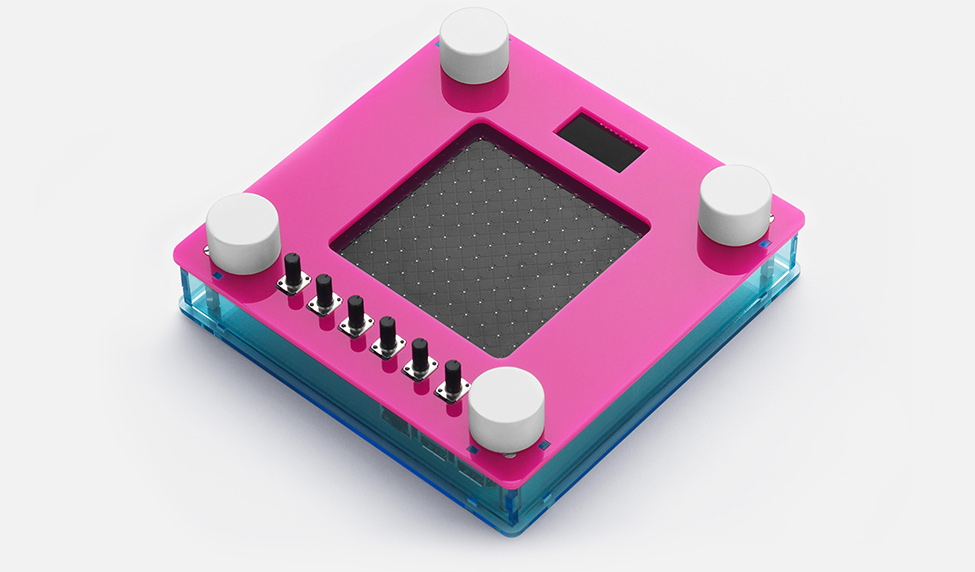
\includegraphics[width=0.5\textwidth]{mt7.jpg}
\end{center}

\subsection*{Boss SY-300}

\begin{itemize}
	\item Supports phone and MIDI input/output
	\item Video: https://youtu.be/dX22RVjdJzw
\end{itemize}

\begin{center}
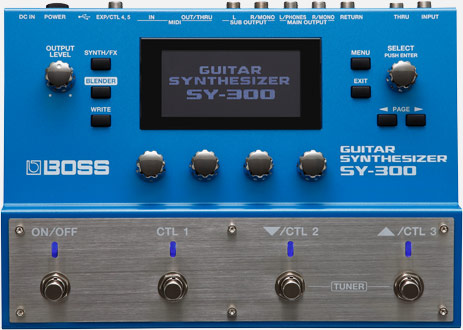
\includegraphics[width=0.5\textwidth]{mt8.jpg}
\end{center}

\end{document}